% @author Arian Helberg

\chapter{Grundlagen}

Die Modellierung mithilfe von Grafiksoftware ist eine vergleichbar händische, langwierige Erstellung von
Objekten.
Hierbei hat der Designer (Modellierer) die volle Kontrolle über die Strukturen des Objektes.\\
Bei der prozeduralen Modellierung werden spezifische Strukturen eines zu erstellenden physikalischen Objektes
generalisiert und meist über eine Grammatik und globale Parameter abgebildet.
Während bei der klassischen Modellierung die menschliche Intuition und bei der prozeduralen Modellierung eine
parametrisierte Grammatik vorausgesetzt wird, arbeitet die inverse prozedurale Modellierung mit bestehenden Modellen und
extrahiert ("`lernt"') die Strukturen des Objektes, die automatisch in eine formale Grammatik überführt werden können.
Die Generierung von prozeduralen Modellen ist ein wichtiges, offenes Problem~\cite{benes_2011}.

\section{Grundbegriffe}

\subsection*{Modellierung}
Um einen physikalischen Körper in ein digitales Objekt zu überführen, wird mithilfe von Abstraktion (Modellierung)
ein mathematisches Modell erstellt, das diesen Körper formal beschreibt.
3D Grafiksoftware, wie bspw. Blender~\cite{blender}, wird genutzt um geometrische Körper zu modellieren, texturieren
und zu animieren.

\newpage

\subsection*{Prozedurale Modellierung}
\begin{quote}
    "`It encompasses a wide variety of generative techniques that
    can (semi-−)automatically produce a specific type of content based on a set of input
    parameters"'~\cite{smelik_2014}
\end{quote}
Prozedurale Modellierung beschreibt generative Techniken, die \\(semi-)automatisch spezifische, digitale
Inhalte anhand von deskriptiven Parametern erzeugen.
\citeauthor{smelik_2014} beschreibt einen Prozess, welcher durch das Nutzen globaler Parameter und descriptiven Regeln
Modelle erzeugt~\cite{smelik_2014}.
\subsection*{Inverse prozedurale Modellierung}
\citeauthor{aliaga_2016} spricht bei der inversen prozeduralen Modellierung von dem Finden einer prozeduralen Repräsentation
von Strukturen bestehender Modelle~\cite{aliaga_2016}.
Die Methodik aus Strukturen bestimmte Regeln und Parameter abzuleiten ist der Hauptgegenstand dieses Feldes der
Computergrafik und aktueller Gegenstand der Forschung.

\section{Grundlegende Arbeiten}

\citeauthor{smelik_2014} untersucht prozedurale Methoden, um diverse Strukturen, wie Vegetation, Straßen u.v.m zu erzeugen.
Es wird ein Überblick aktueller, vielversprechender Studien gegeben, deren Anwendung sowohl in technischen Bereichen,
als auch in nicht-technischen, kreativen Bereichen, diskutiert wird.~\cite{smelik_2014} gilt als grundlegender Einstiegspunkt
in die Bereiche der prozeduralen Modellierung.
Einen aktuellen Stand der Forschung der inversen prozeduralen Modellierung liefert~\cite{aliaga_2016}.~\Citeauthor{aliaga_2016}
zeigt, dass IPM-Ansätze in entsprechende Kernprobleme der Informatik aufgeteilt und meist getrennt voneinander durch
verschiedene Methodiken und Algorithmen bearbeitet werden.
Weiter wird ein Einblick in die Kategorisierung und Bewertung einiger Ergebnisse von IPM-Systemem gegeben.
Die Buchrezension~\cite{daelemans_2010} geht auf die Arbeit~\cite{higuera_2010} ein und weist darauf hin, dass~\citeauthor{higuera_2010}
einen wesentlichen Unterschied zwischen der Induktion einer Grammatik und der Grammatikinferrierung sieht.
Die Induktion beschreibt das Finden einer Grammatik, welche ein Datum am genauesten beschreibt.
Die Gammatikinferierung ist das Finden einer Grammatik, die eine bestimmte Zeichenfolge abdeckt.

\newpage

\citeauthor{higuera_2010} ordnet die inverse Generierung von L-Systemen zum Problem der Grammatikinferrenz, welches er
als gut erforschtes Gebiet beschreibt.
Verzweigungsstrukturen im Kontext der inversen prozeduralen Modellierung tauchen in wissenschaftlichen Studien wenig auf.
~\cite{guo_2020} adressiert diese in seiner Arbeit~\cite{guo_2020} und liefert einige Ansätze hierzu.\\~\\

Im Folgenden wird eine Übersicht zu einigen Arbeiten zur Modellierung von bestimmten Strukturen gegeben.
\begin{center}
    \begin{tabular}{l|l|l|l}
        Subjekt & Autor & Jahr & Arbeit\\
        \hline
        Bäume und Landschaften & ~\citeauthor{deussen_2010} & 2010 & ~\cite{deussen_2010} \\
        Fassaden & ~\citeauthor{alhalawani_2013} & 2016 & ~\cite{alhalawani_2013} \\
        Gebäude & ~\citeauthor{mueller_2006} & 2006 & ~\cite{mueller_2006} \\
        Städte & ~\citeauthor{parish_2001} & 2001 & ~\cite{parish_2001} \\
        Möbel & ~\citeauthor{merrell_2011} & 2011 &  ~\cite{merrell_2011} \\
        Inneneinrichtung & ~\citeauthor{zhang_2019} & 2019 & ~\cite{zhang_2019} \\
    \end{tabular}
\end{center}

\subsection*{L-Systeme}
\citeauthor{lindemayer_1968} führt eine mathematische Beschreibung zum Wachstum fadenförmiger Organismen ein.
Sie zeigt, wie sich der Status von Zellen infolge ein oder mehrerer Einflüsse verhält~\cite{lindemayer_1968}.
Weiter führt er Ersetzungssysteme ein, die atomare Teile mithilfe von Produktionsregeln ersetzen.
Diese L-Systeme nutzt er zur formalen Beschreibung von Zellteilung.
Später werden Symbole zur formalen Beschreibung von Verzweigungen, die von Filamenten abgehen, eingeführt~\cite{prusinkiewicz_1990}.
Die bekanntesten L-Systeme sind zeichenketten-basiert und werden von \textit{Noam Chomsky} in~\cite{chomsky_1956} eingeführt.
Sie ersetzen parallel Symbole eines Wortes, die von einer Grammatik über eine Sprache akzeptiert werden.
L-Systeme können unter anderem parametrisiert oder nicht-parametrisiert und kontextfrei oder kontextsensitiv sein.

\newpage

L-Systeme sind Grammatiken mit folgender Form:
\begin{center}
    $\mathcal{L}=\langle M,\omega,R \rangle$, mit
    \begin{itemize}
        \item $M$ als Alphabet, das alle Symbole enthält, die in der Grammatik vorkommen,
        \item $\omega$ als Axiom oder "`Startwort"' und
        \item $R$ als Menge aller Produktionsregeln, die für $\mathcal{L}$ gelten
    \end{itemize}
\end{center}
Das Alphabet eines parametrisierten Systems enthält Module (Symbole mit Parametern) anstatt Symbole:
\begin{center}
    $M=\{A(P),B(P),\dots\}$ mit
    \begin{itemize}
        \item $P=p_1,p_2,\dots$ als Modulparameter
    \end{itemize}
\end{center}
Zeichen des Alphabets, die Ziel einer Produktionsregel sind, heißen Variablen.
Alle anderen Zeichen aus $M$ sind Konstanten.
Das Axiom $\omega$ ist eine nicht-leere Sequenz an Modulen aus $M^+$ mit
\begin{itemize}
    \item $M^+$ als Menge aller möglichen Zeichenketten aus Modulen aus $M$
\end{itemize}
Produktionsregeln sind geordnete Paare aus Wörtern über dem Alphabet, die bestimmte Ersetzungsregeln umsetzen.
Hierbei werden Symbole aus einem Wort, die einer rechten Seite (\textit{engl. right hand side (RHS)}) einer
Produktionsregel entsprechen, durch die linke Seite des Paares (\textit{engl. left hand side (LHS)}) ersetzt.
Sie sind folgendermaßen aufgabaut:
\begin{center}
    $A(P)\rightarrow x,x\in M^*$, mit
    \begin{itemize}
        \item $M^*$ als die Menge aller möglichen Zeichenketten von M inklusive der leeren Zeichenkette $\varepsilon$
    \end{itemize}
\end{center}
Ist die RHS jeder Produktionsregel ein einzelnes Symbol und gibt es zu jeder Variablen eine Regel, spricht man
von einem kontextfreien, andernfalls von einem kontextsensitiven L-System.

\subsubsection*{L-System Interpretation}
Lindenmayer-Systeme können Worte über ihr Alphabet interpretieren.
Dafür werden Symbole des Wortes, die Ziel einer Produktionsregeln sind, in Iterationen durch die RHS
der Produktionsregeln ersetzt.
Bei der Ausführung eines L-Systems wird kein beliebiges Wort interpretiert, sondern das in der
Grammatik definierte Axiom.

\subsection*{Logo-Turtle-Algorithmus}
Der Logo-Turtle-Algorithmus~\cite{prusinkiewicz_1986} setzt ein Vorgehen zur graphischen Beschreibung von L-Systemen, bei dem
jeder Buchstabe in einem Wort einer bestimmten Zeichenoperation zugewiesen wird, um.
So kann aus einem L-System ein grafisches Muster generiert werden, das mit einer Abfolge von Zeichenbefehlen an
eine "`Schildkröte"' gezeichnet wird.
Das Triplett $(x,y,\theta)$ definiert den Status (State) der Schildkröte.
Dieser setzt sich aus der aktuellen Position $\left(\begin{smallmatrix} x \\ y \end{smallmatrix}\right)$ und dem
aktuellen Rotationswinkel $\theta$, der die Blickrichtung bestimmt, zusammen.\\
Der Algorithmus kann als Komprimierung eines geometrischen Musters gesehen werden.
Symbole mit zugehörigen Steuerungsbefehlen und Statusveränderung:
\begin{center}
    \begin{tabular}{lll}
        % ROW 1
        \textbf{Symbol} & \textbf{Steuerung} & \textbf{Statusveränderung} \\
        \hline \\
        % ROW 2
        $F(d)$ &
        \begin{minipage}{0.6\textwidth}
            Gehe vom derzeitigen Punkt $p_1$ $d$ Einheiten in die Blickrichtung zu dem Punkt $p_2$.
            Zeichne ein Liniensegment zwischen $p_1$ und $p_2$\\
        \end{minipage} &
        ja
        \\ \hline \\
        % ROW 3
        $+(\alpha)$ &
        \begin{minipage}{0.6\textwidth}
            Setze neuen Rotationswinkel $\theta=\theta+\alpha$\\
        \end{minipage} &
        ja
        \\ \hline \\
        % ROW 4
        $-(\alpha)$ &
        \begin{minipage}{0.6\textwidth}
            Setze neuen Rotationswinkel $\theta=\theta-\alpha$\\
        \end{minipage} &
        ja
        \\ \hline \\
        % ROW 5
        $[$ &
        \begin{minipage}{0.6\textwidth}
            Lege den aktuellen State auf einen Stack\\
        \end{minipage} &
        nein
        \\ \hline \\
        % ROW 6
        $]$ &
        \begin{minipage}{0.6\textwidth}
            Hole den State vom Stack und überschreibe den aktuellen mit diesem\\
        \end{minipage} &
        nein
    \end{tabular}
\end{center}

\subsection*{Extreme Programming}
Eine Fallstudie der Universität Karlsruhe~\cite{muller_2001} untersucht den Einsatz der Softwaretechnik Extreme
Programming (XP) im Kontext der Erstellung von Abschlussarbeiten im Universitätsumfeld.
Hierzu werden folgende Schlüsselpraktiken untersucht:
\begin{itemize}
    \item XP als Softwaretechnik zur schrittweisen Annäherung an die Anforderungen eines Systems
    \item Änderung der Anforderungen an das Systems
    \item Funktionalitäten (Features) werden als Tätigkeiten des Benutzers (User Stories) definiert
    \item Zuerst werden Komponententests (Modultests) geschrieben und anschließend die Features (Test-driven Design)
    \item Keine seperaten Testing-Phasen
    \item Keine formalen Reviews oder Inspektionen
    \item Regelmäßige Integration von Änderungen
    \item Gemeinsame Implementierung (Pair Programming) in Zweiergruppen
\end{itemize}
Aus der Fallstudie geht hervor, dass Extreme Programming einige Vorteile bei der Bearbeitung eines Softwareprojektes
einer Bachelorarbeit bietet.
Zum Einen können sich Anforderungen an das zu erstellende System durch parallele Literaturrecherche ändern, zum
Anderen können Arbeitspakete durch Releases abgebildet werden.
Diese Softwaretechnik wird in der Umsetzung des Softwareprojekts zu dieser Arbeit angewendet.

\begin{figure}[H]
    \centering
    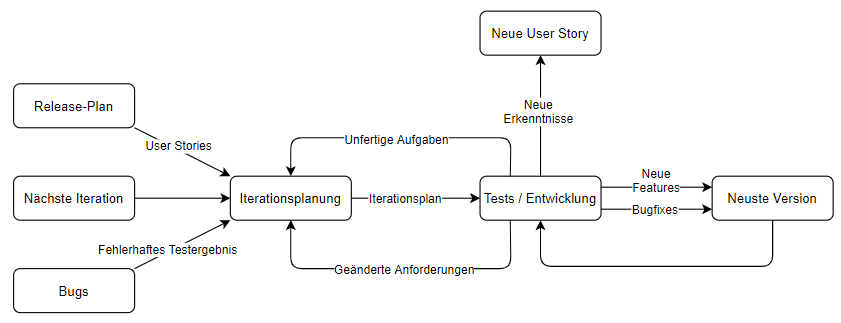
\includegraphics[width=12.8cm]{../images/extreme_programming.png}
    \caption{Zyklische Umsetzung des Softwareprojektes}
\end{figure}

\section{Verwandte Arbeiten}

\citeauthor{guo_2020} führt ein Modell zum Lernen von L-Systemen von Verzweigungsstrukturen mithilfe maschinellen
Lernens (Deep Learning) anhand beliebiger Grafiken ein~\cite{guo_2020}.
Hierzu werden atomare Strukturen mit einem neuronalen Netz erkannt, eine hierarchische Topologie (Baumstruktur)
aufgebaut, aus der ein L-System inferiert und mit einem Greedy Algorithmus optimiert wird.
Ausgabe des Systems ist ein generalisiertes L-System, aus dem ähnliche Strukturen, wie die der Inputgrafik,
erstellt werden können.\\
Das Lernen von Design-Patterns mithilfe von Bayes-Grammatiken ist Gegenstand der Arbeit von~\citeauthor{talton_2012}.
~\cite{talton_2012} führt ein System zur Generierung geometrischer Modelle und Websites ein, das eine organisierte
Struktur von bezeichneten Teilmodellen entgegennimmt und über einen Prozess der MCMC-Optimierung eine Bayes-optimale
Grammatik erstellt, um neue Modelle zu generieren.\\
Auch ~\cite{stava_2014} etabliert einen MCMC-Ansatz zum Finden prozeduraler Repräsentationen für biologische Bäume.
Hier wird zunächst über eine Laplace-Glättung ein Grundgerüst gefunden, das dann in einer Baumtopologie organisiert wird.\\
Das von ~\citeauthor{martinovic_2013} eingeführte System nutzt ähnlich organisierte Eingabestrukturen in Form von
Gebäudefassaden, um durch bayesische Grammatikinduktion eine kontextfreie Grammatik zu induzieren ~\cite{martinovic_2013}.
Das Erstellen kontextfreier Grammatiken mithilfe statistischer Methoden zur Verteilung von zweidimensionalen Clustern
wird in den Arbeit von ~\citeauthor{stava_2010} gegeben.

%urbanen Strukturen~\cite{nishida_2016}
%Polynomiale Algorithmen zum Inferieren von L-Systemen~\cite{mcquillan_2018}
%Framework zum Inferieren von L-Systemen aus Vektordaten~\cite{stava_2010}
%Generalisieren einen Regelsets aus einem Inputset mit Markov Chain Monte Carlo~\cite{talton_2012, talton_2011}
%Lernen von Regeln zum Layout für Gebäude~\cite{martinovic_2013}
%Inverse prozedurale Modellierung von Fassaden~\cite{xiao_2008}